\documentclass[a4paper,12pt]{article}
\usepackage{inconsolata}
\usepackage{listings}
\usepackage[margin=2cm]{geometry}
\usepackage[LGR, T1]{fontenc}
\usepackage[utf8]{inputenc}
\usepackage[greek, english]{babel}
\usepackage{alphabeta}
\usepackage{amsfonts}
\usepackage{amsmath}
\usepackage{amssymb}
\usepackage{fixltx2e}
\usepackage{subfig}
\usepackage{float}
\usepackage{xcolor}
\usepackage{listings}
\usepackage{graphicx}
\definecolor{codeblue}{RGB}{44,133,217}
\definecolor{codegray}{RGB}{138,150,150}
\definecolor{codepurple}{RGB}{0.58,0,0.82}
\definecolor{backcolour}{RGB}{255,255,255}
\lstdefinestyle{mystyle}{
    backgroundcolor=\color{backcolour},
    commentstyle=\color{codegray},
    keywordstyle=\color{codeblue},
    numberstyle=\color{codegray}\ttfamily\bfseries,
    stringstyle=\color{codepurple},
    basicstyle=\ttfamily\small\bfseries,
    breakatwhitespace=false,
    breaklines=true,
    captionpos=b,
    keepspaces=true,
    numbers=left,
    numbersep=5pt,
    showspaces=true,
    showstringspaces=false,
    showtabs=false,
    tabsize=2
}
\lstset{style=mystyle}
\begin{document}
\begin{titlepage}
    \begin{center}
        \vspace*{\fill}
        \huge{\textbf{Αριθμητική Γραμμική Άλγεβρα\\}}
        \vfill
        \huge{\textbf{Project 1}}
        \vspace*{\fill}
        \vfill
        \normalsize\textbf{Ζαμάγιας Μιχάλης\\}
        \small\textbf{Εαρινό Εξάμηνο, 2020\\}
        \vfill
    \end{center}
\end{titlepage}
\tableofcontents
\newpage\section{Άσκηση 1}
\subsection{Εκφώνηση}
Φτιάξτε ένα πρόγραμμα σε Octave που να δέχεται έναν ${2x2}$ συμμετρικό πίνακα ως δεδομένα και να
υπολογίζει το χαρακτηριστικό πολυώνυμο του πίνακα. Κάντε το να βρίσκει τις ιδιοτιμές του πίνακα
λύνοντας το χαρακτηριστικό πολυώνυμο και μετά, για κάθε ιδιοτιμή να βρίσκει ένα μοναδιαίο ιδιοδιάνυσμα
λύνοντας μία από τις εξισώσεις που δίνουν το ιδιοδιάνυσμα. Επαληθεύστε τα αποτελέσματα του προγράμματός
σας δίνοντας την έτοιμη εντολή διαγονοποίησης "eig" που έχει το Octave. Δώστε τα αποτελέσματα του
προγράμματός σας στον πίνακα
$
    A=\begin{pmatrix}
        1 & 2 \\
        2 & 1
    \end{pmatrix}
$
και
$
    A=\begin{pmatrix}
        1   & \mu \\
        \mu & 1
    \end{pmatrix}
$
. Εδώ ${\mu}$ είναι το τελευταίο ψηφίο του αριθμού μητρώου σας.
\subsection{Απάντηση}
Ακολουθεί το αποτέλεσμα για τον πίνακα
$
    A=\begin{pmatrix}
        1 & 2 \\
        2 & 1
    \end{pmatrix}
$
:
\lstinputlisting[firstline=2, lastline=48]{"Task 1.txt"}
Ο πίνακας
$
    A=\begin{pmatrix}
        1   & \mu \\
        \mu & 1
    \end{pmatrix}
$
για μένα είναι ο ταυτοτικός, επειδή έχω 5000 για αριθμό μητρώου. Δίνει το εξής αποτέλεσμα:
\lstinputlisting[firstline=55, lastline=91]{"Task 1.txt"}
Όπως παρατηρείται στην γραμμή 31, το σύστημα φαίνεται να μην δίνει λύσεις. Όμως, βάσει θεωρίας:
\begin{equation}
    \begin{split}
        A - \lambda I &= 0 \\
        A &= \lambda I \\
        I &= \lambda I \\
        \lambda & =\frac{I}{I} \\
        \lambda & =1
    \end{split}
\end{equation}
έχουμε εύκολα ότι η ιδιοτιμή του ταυτοτικού  πίνακα Α ισούται με 1, κι έχουμε:
\begin{equation}
    \begin{split}
        A v &= \lambda v \\
        I v&= 1 v \\
    \end{split}
\end{equation}
Άρα, κάθε διάνυσμα είναι ιδιοδιάνυσμα του Α.
\newpage\section{Άσκηση 2}
\subsection{Εκφώνηση}
Σκοπός της άσκησης είναι να δούμε την δράση ενός συμμετρικού πίνακα A πανω στα διανύσματα θέσης (σημεία)
του επιπέδου. Φτιάξτε ένα πρόγραμμα που θα δέχεται ένα διάνυσμα
$
    \begin{pmatrix}
        x \\
        y
    \end{pmatrix}
$
στο επίπεδο και θα το μετασχηματίζει στο διάνυσμα
$
    A
    \begin{pmatrix}
        x \\
        y
    \end{pmatrix}
$
. Για την γραφική απεικόνιση των δύο διανυσμάτων, ζωγραφίσετε μία μπλε γραμμή από την αρχή των αξόνων
στο σημείο
$
    \begin{pmatrix}
        x \\
        y
    \end{pmatrix}
$
, και μία κόκκινη γραμμή από την αρχή των αξόνων στο σημείο
$
    A
    \begin{pmatrix}
        x \\
        y
    \end{pmatrix}
$. Δώστε τα αποτελέσματα σας για
$
    A=\begin{pmatrix}
        1 & 2 \\
        2 & 1
    \end{pmatrix}
$
και για
$
    \begin{pmatrix}
        x \\
        y
    \end{pmatrix}=\begin{pmatrix}
        1 \\
        0
    \end{pmatrix}
$
, καθώς και για
$
    \begin{pmatrix}
        x \\
        y
    \end{pmatrix}=\begin{pmatrix}
        0 \\
        1
    \end{pmatrix}
$
. Ποια είναι η σχέση των μετασχηματισμένων διανυσμάτων με τον πίνακα Α;
\subsection{Απάντηση}
Έξοδος προγράμματος:
\lstinputlisting[firstline=1, lastline=25]{"Task 2.txt"}
Τα γραφήματα:
\begin{figure}
    \centering
    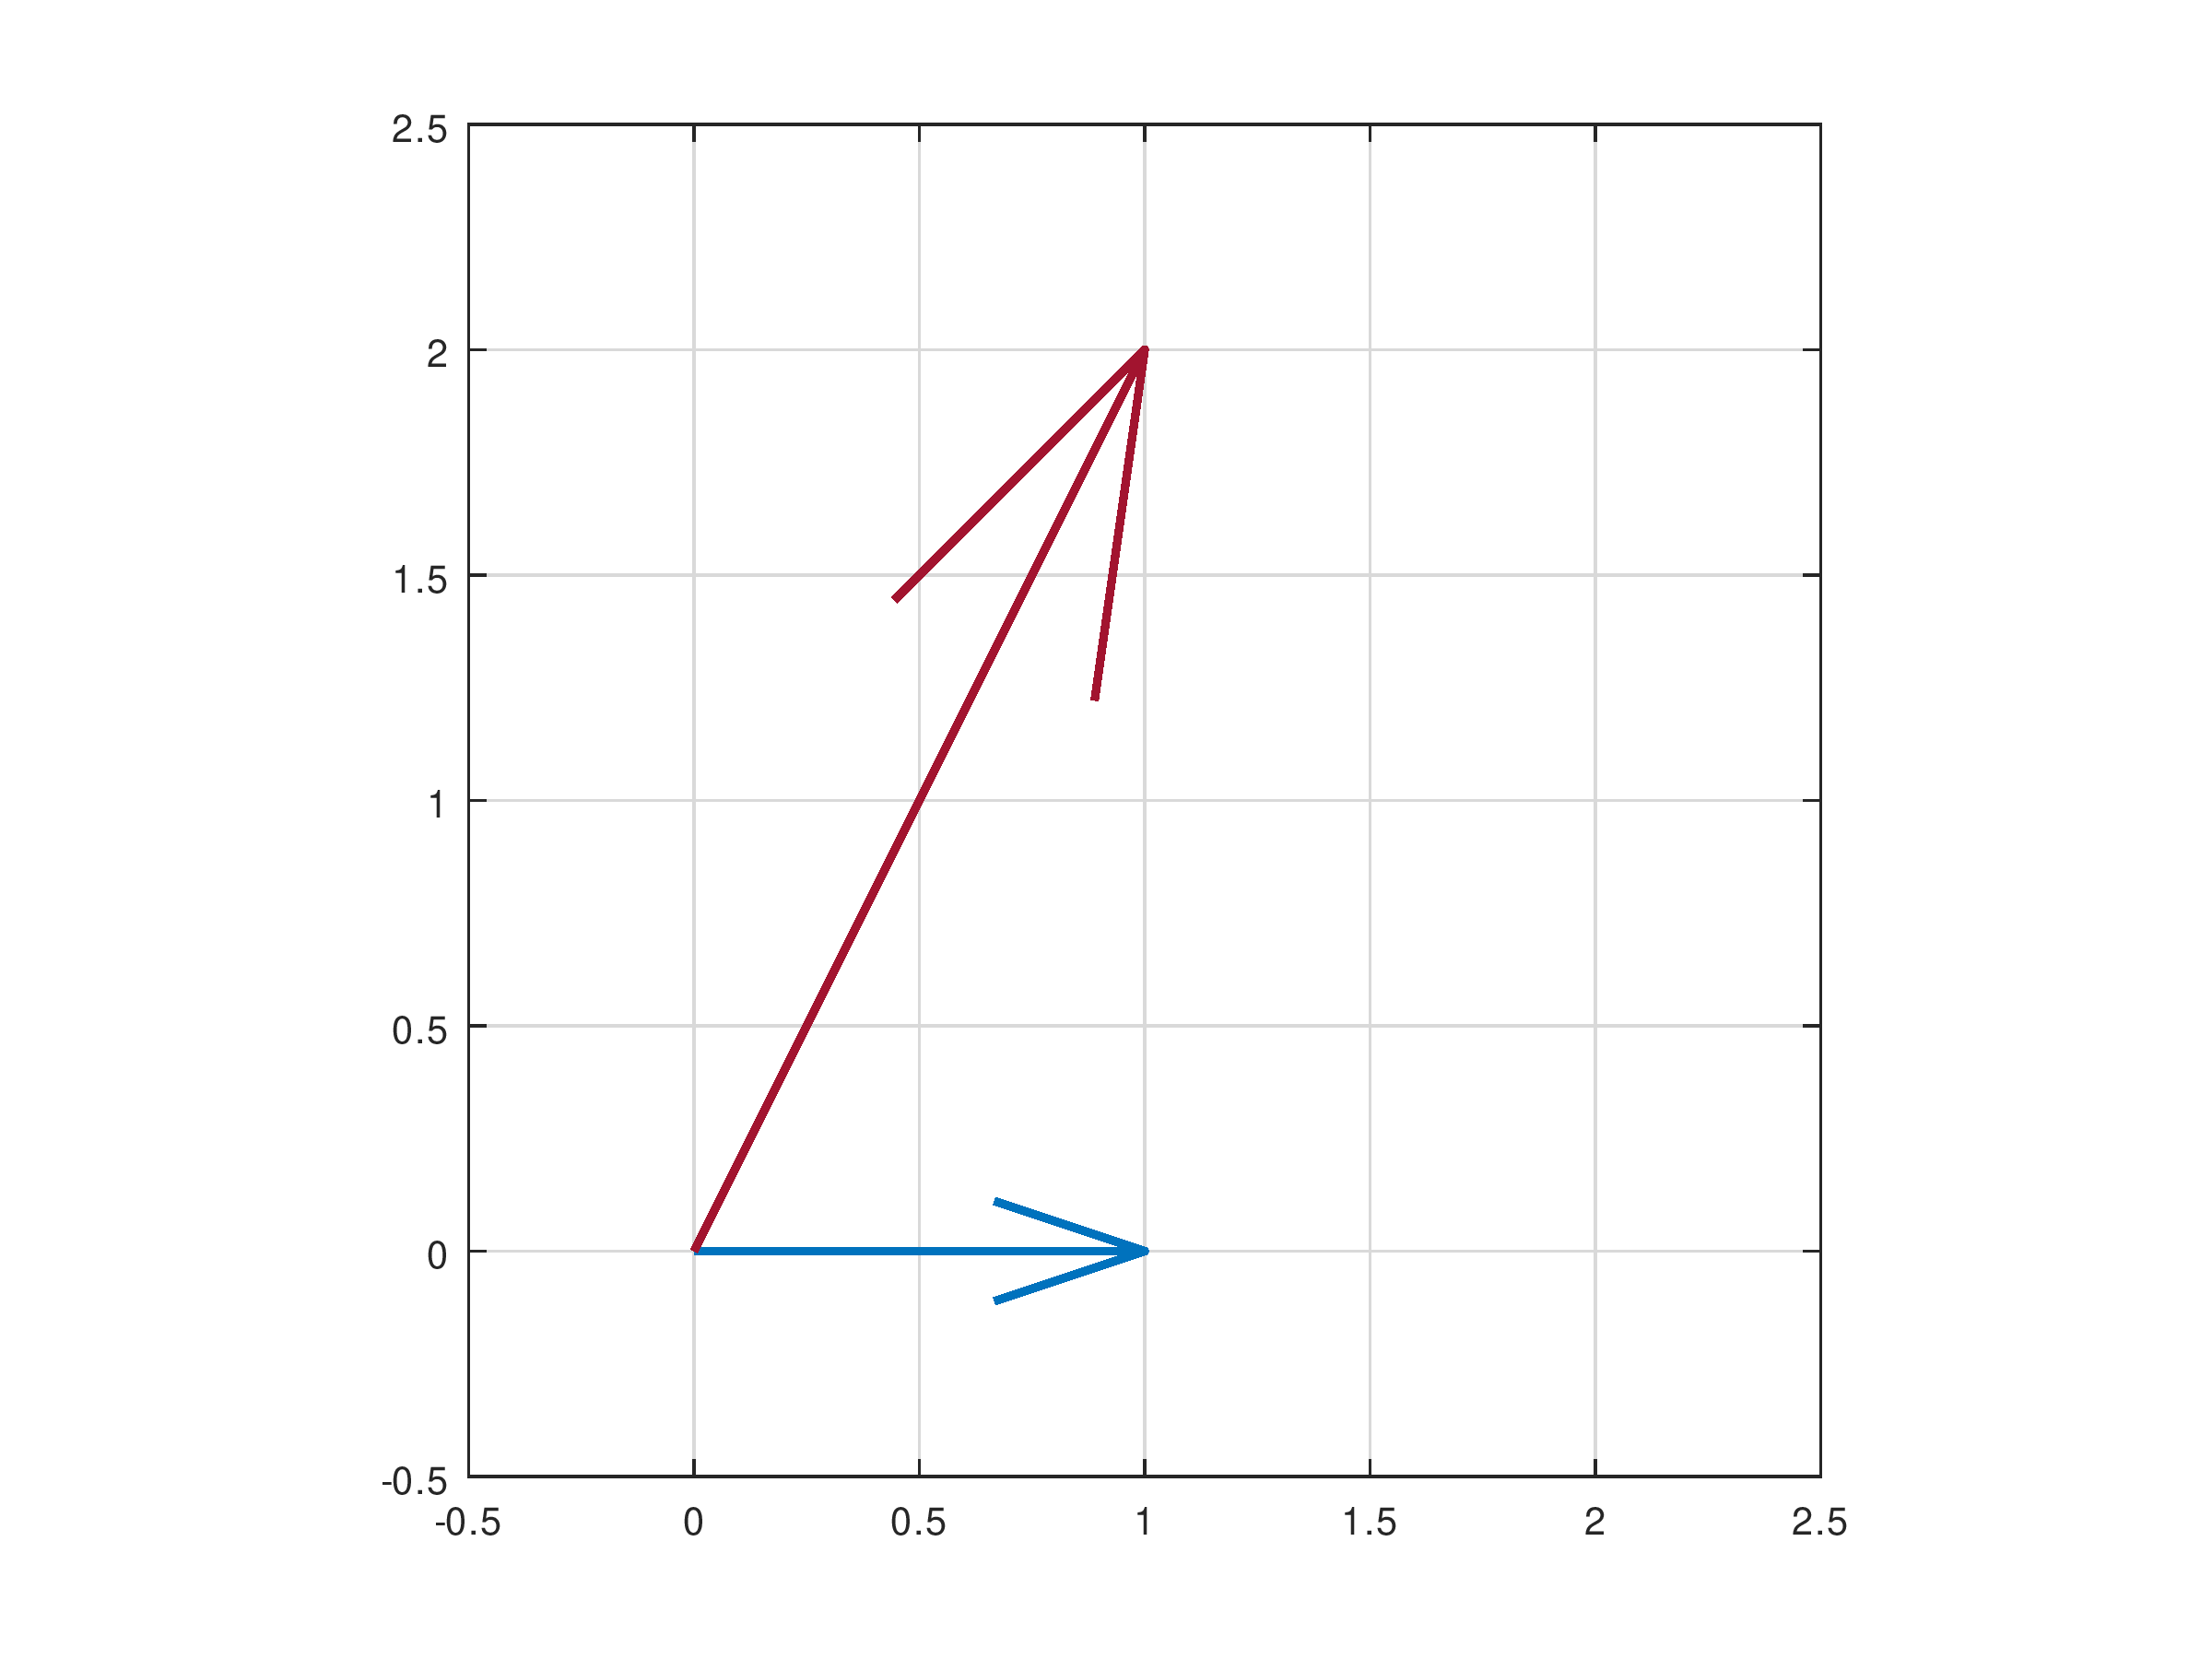
\includegraphics[scale=0.6]{x1.png}
    \caption{φαίνεται Με μπλέ το αρχικό διάνυσμα
        $
            \begin{pmatrix}
                1 \\
                0
            \end{pmatrix}
        $
        και με κόκκινο ο μετασχηματισμός του σε
        $
            \text{A} \begin{pmatrix}
                1 \\
                0
            \end{pmatrix}
        $
        .}
\end{figure}
\begin{figure}
    \centering
    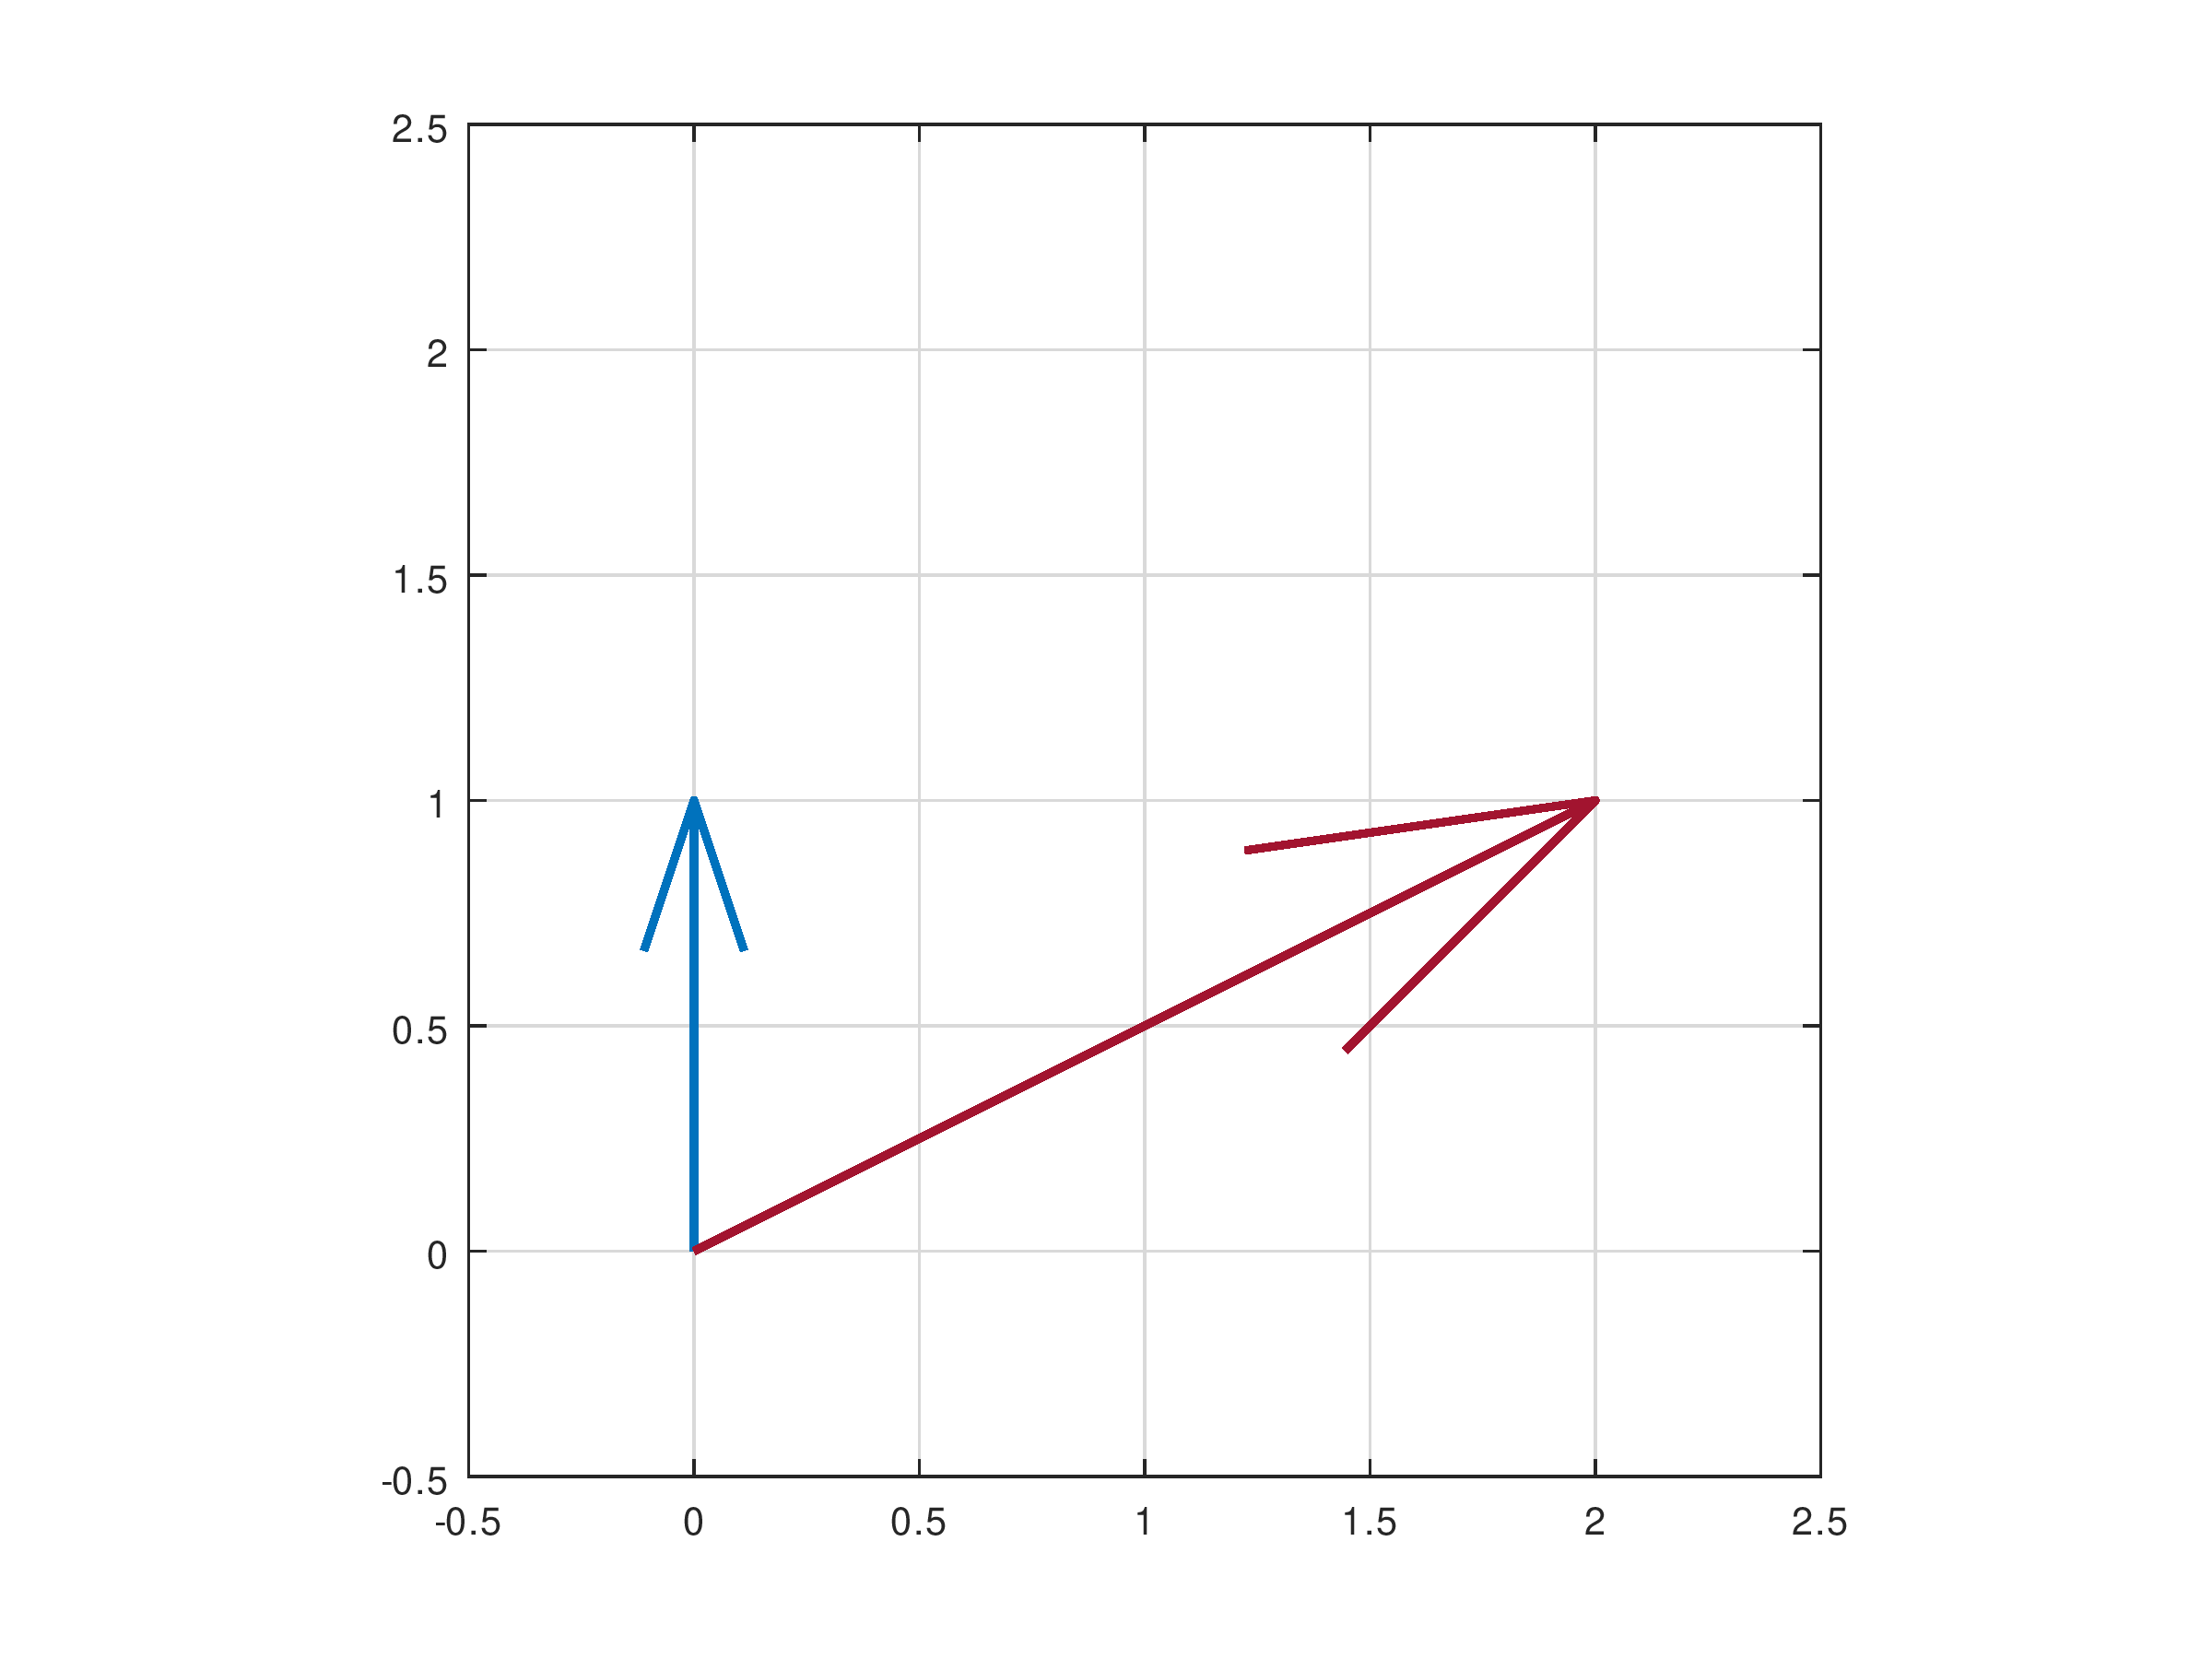
\includegraphics[scale=0.6]{x2.png}
    \caption{Φαίνεται με μπλε το αρχικό διάνυσμα
        $
            \begin{pmatrix}
                0 \\
                1
            \end{pmatrix}
        $
        και με κόκκινο ο μετασχηματισμός του σε
        $
            \text{A} \begin{pmatrix}
                0 \\
                1
            \end{pmatrix}
        $.}
\end{figure}
\newpage\section{Άσκηση 3}
\subsection{Εκφώνηση}
Σκοπός της άσκησης είναι να δούμε πως δρα ένας συμμετρικός πίνακας Α σε μία καμπύλη στο επίπεδο.
Για αυτόν τον σκοπό θα ζωγραφίσετε (με Octave) ένα μοναδιαίο κύκλο στο επίπεδο με μπλε χρώμα.
Για να επιτευχθεί εύκολα αυτό χρησιμοποιήστε την παραμετρική μορφή του μοναδιαίου κύκλου, $x=\cos{t}$,
$y=\sin{t}$. Μετά θα μετασχηματίσετε τον κύκλο σύμφωνα με τον πίνακα Α, μετασχηματίζοντας όλα τα σημεία
του με τον πίνακα Α. Εν γένη, από αυτόν τον μετασχηματισμό προκύπτει μια έλλειψη. Αυτήν την έλλειψη θα την
ζωγραφίσετε με κόκκινο χρώμα στο ίδιο σύστημα αξόνων με τον κύκλο. Δώστε τα αποτελέσματά σας για
$
    A=\begin{pmatrix}
        1 & 2 \\
        2 & 1
    \end{pmatrix}
$
και
$
    A=\begin{pmatrix}
        1   & \mu \\
        \mu & 1
    \end{pmatrix}
$
.
\subsection{Απάντηση}
Έξοδος προγράμματος:
\lstinputlisting[firstline=2, lastline=29]{"Task 3.txt"}
Χρησιμοποιείται το πακέτο symbolic για να δούμε τον μετασχηματισμό των σημείων του κύκλου από
την επίδραση των πινάκων Α.
Παρατειρείται ξανά, ο πίνακας
$
    A = \begin{pmatrix}
        1   & \mu \\
        \mu & 1
    \end{pmatrix}
$
, όπου $\mu = 0$, είναι ταυτοτικός με αποτέλεσμα ο μετασχηματισμός του κύκλου να είναι ο κύκλος
με τα ίδια δεδομένα με τον αρχίκο, κέντρο την αρχή των αξόνων και ακτίνα ίση με την μονάδα.
\begin{figure}
    \centering
    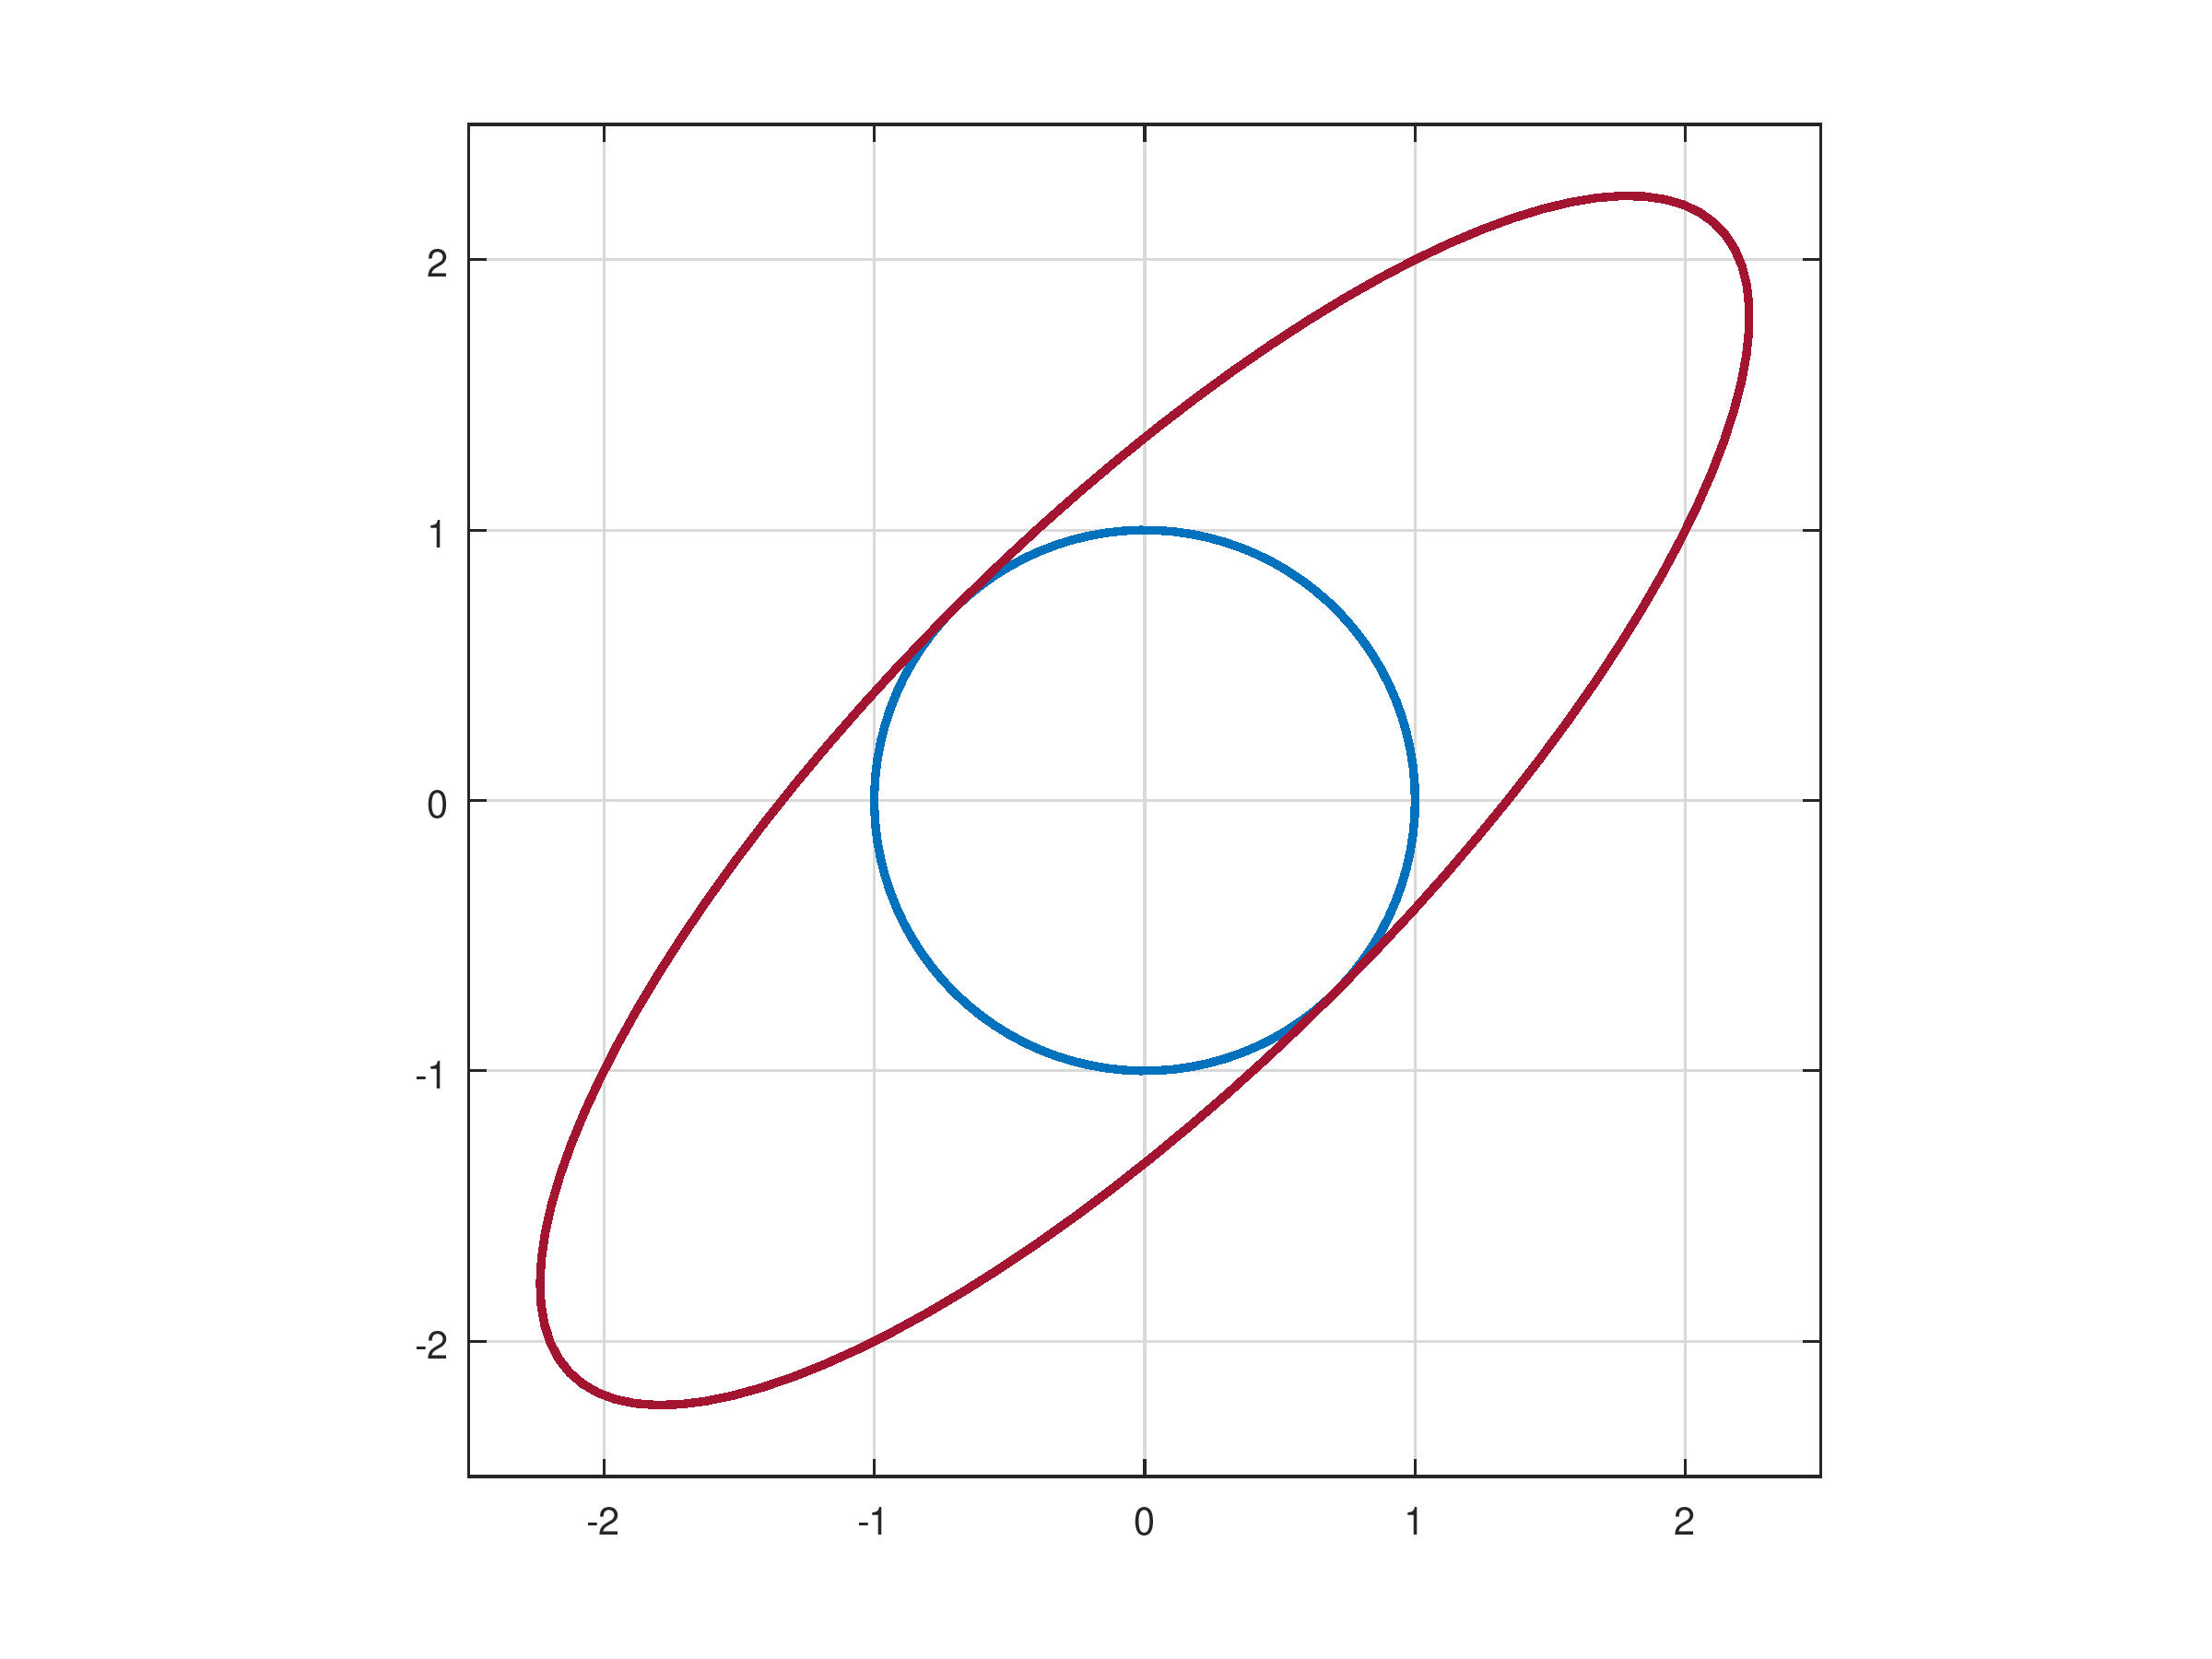
\includegraphics[scale=0.6]{a.png}
    \caption{Φαίνεται με μπλε ο αρχικός κύκλος και με κόκκινο η έλλειψη που προκύπτει από τον
        μετασχηματισμό του με τον πίνακα
        $
            A=\begin{pmatrix}
                1 & 2 \\
                2 & 1
            \end{pmatrix}
        $
        .}
\end{figure}
\begin{figure}
    \centering
    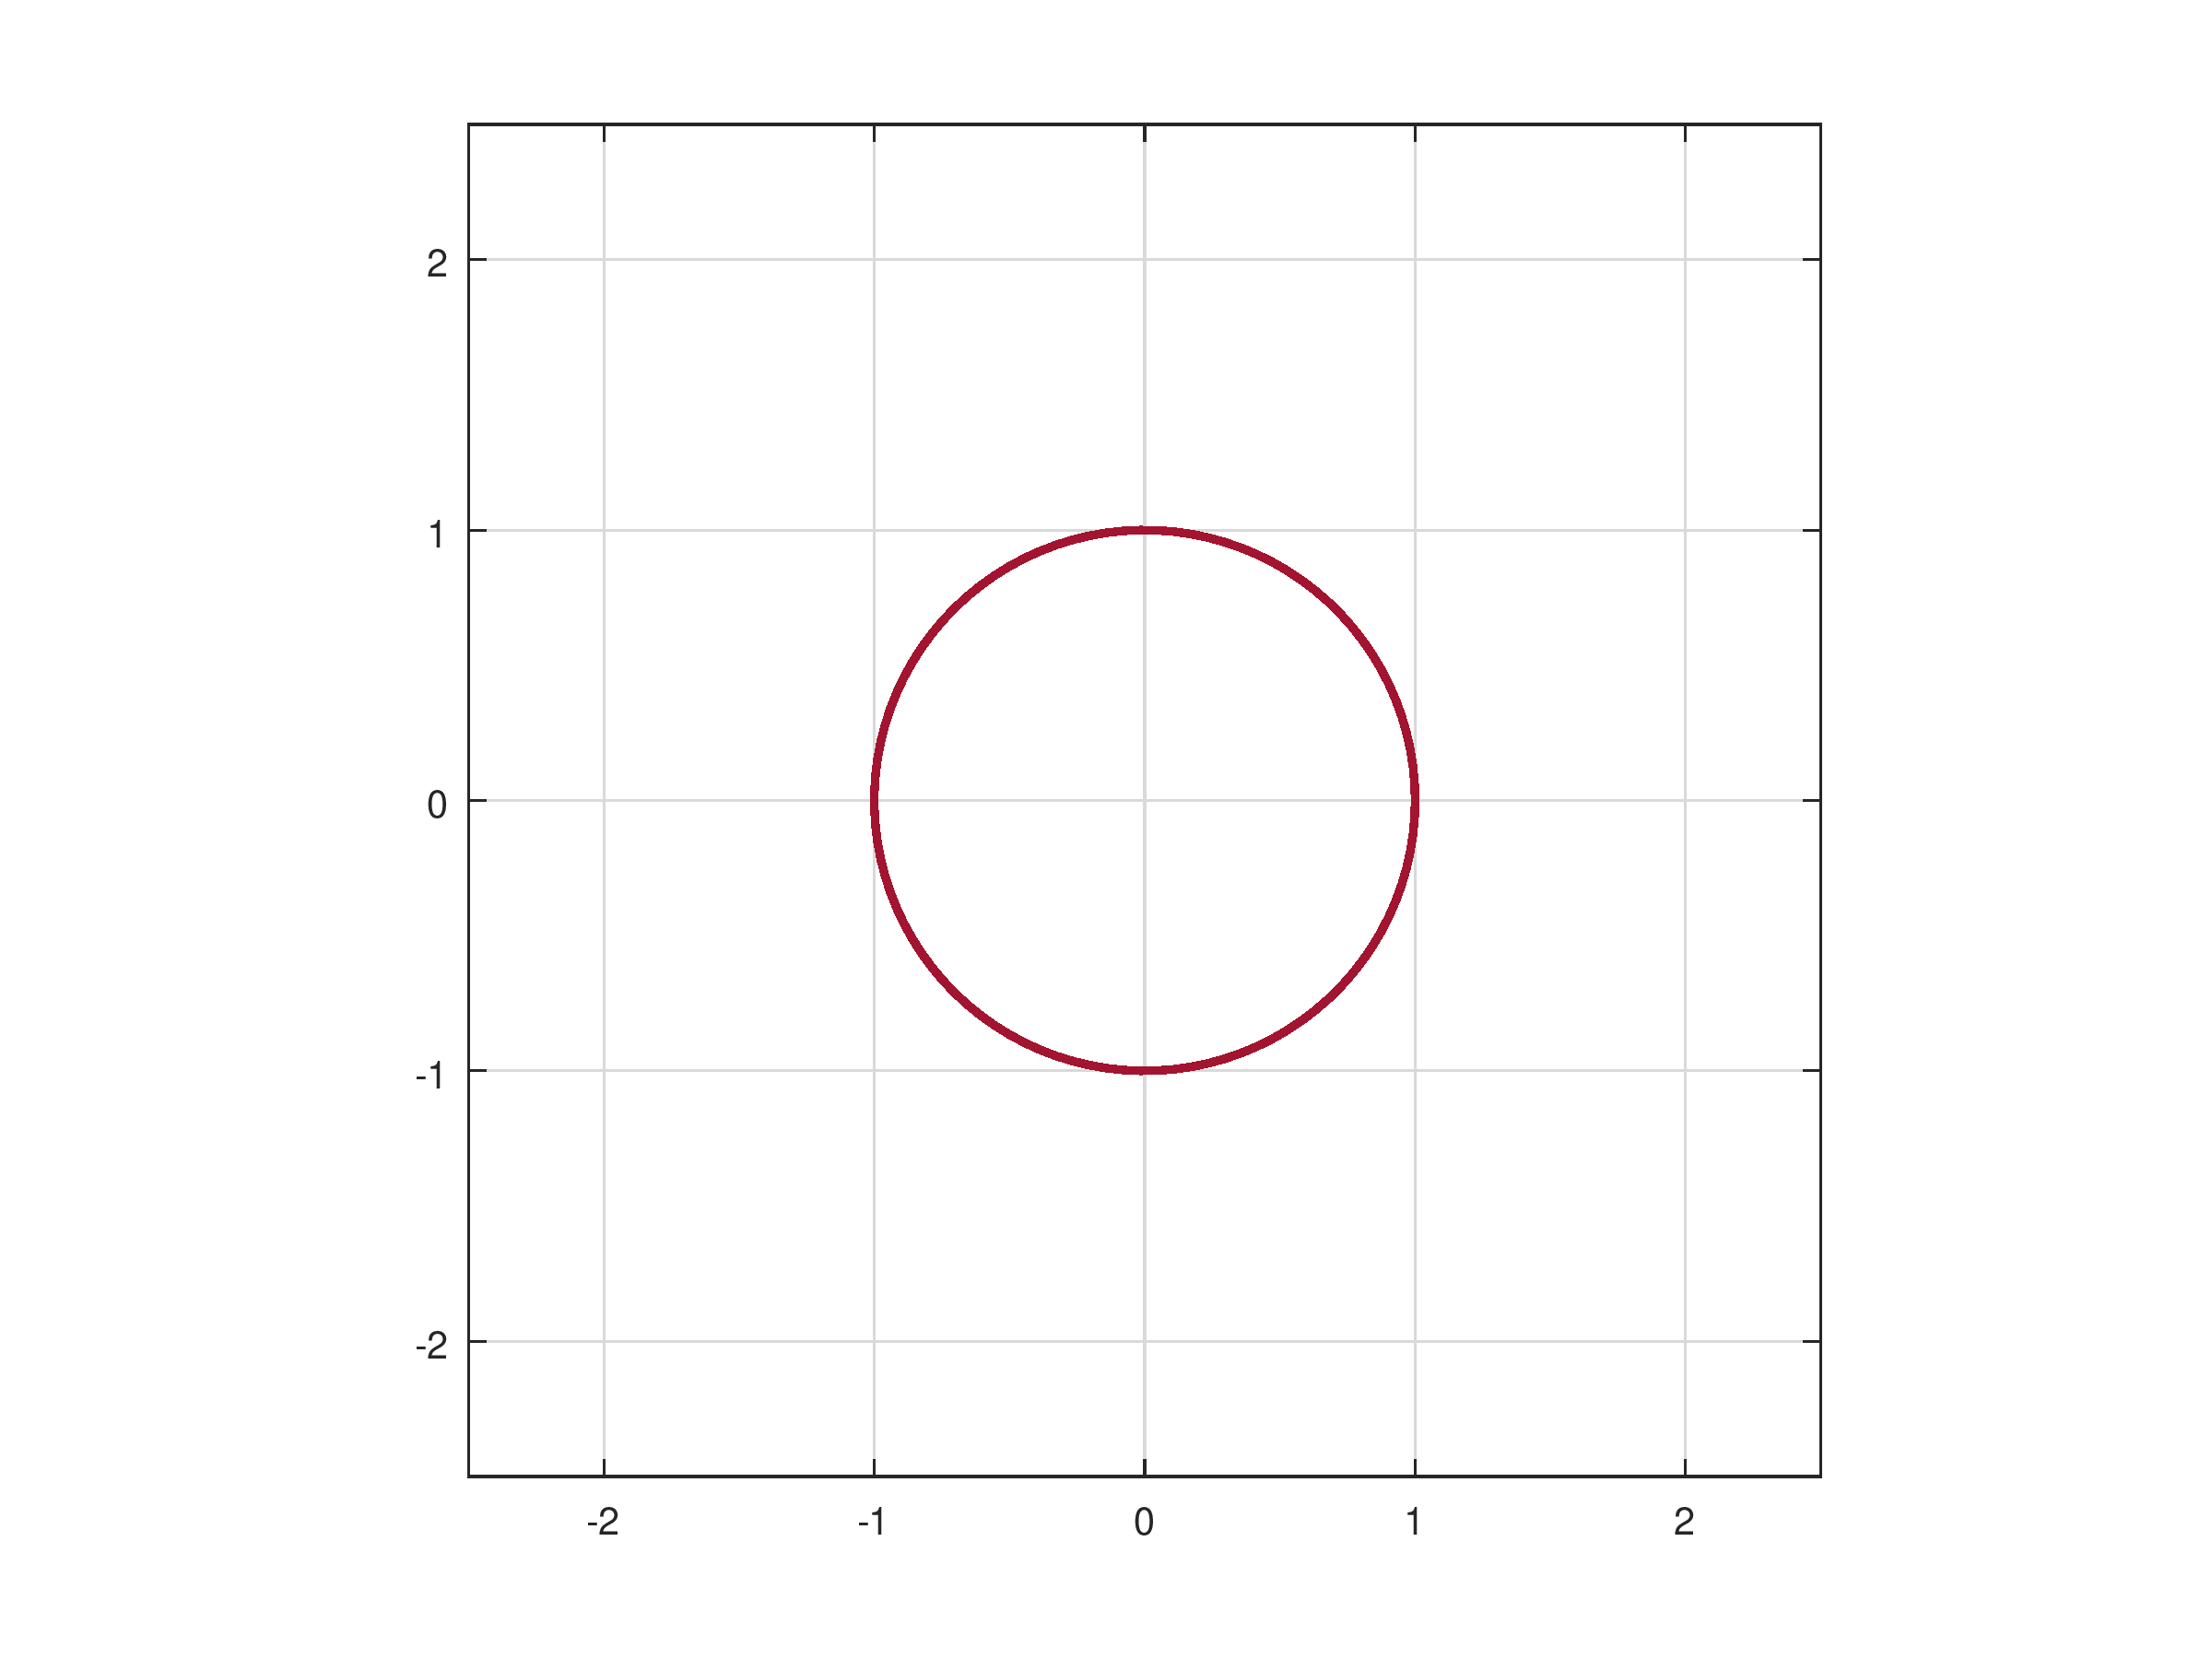
\includegraphics[scale=0.6]{i.png}
    \caption{Φαίνεται με κόκκινο ο μετασχηματισμός του αρχικού κύκλου πάνω από τον αρχικό κύκλο,
        που προκύπτει με την επίδραση του ταυτοτικού πίνακα Α στον αρχικό κύκλο.}
\end{figure}
\newpage\section{Άσκηση 4}
\subsection{Εκφώνηση}
Σκοπός της άσκησης είναι να διαβάσουμε τα ιδιοδιανύσματα από την δράση ενός συμμετρικού πίνακα Α στο
επίπεδο. Πάνω στο γράφημα με τον κύκλο και την έλλειψη της άσκησης 3, ζωγραφίστε και τα ιδιοδιανύσματα
του πίνακα Α ως ευθύγραμμα τμήματα που ξεκινούν από την αρχή τον αξόνων. Το μήκος κάθε ιδιοδιανύσματος
πάρτε το να είναι ίσο με την ιδιοτιμή που αντιστοιχεί με αυτό, κατ' απόλυτη τιμή. Τι παρατηρείτε; Δώστε
τα αποτελέσματά σας για
$
    A=\begin{pmatrix}
        1 & 2 \\
        2 & 1
    \end{pmatrix}
$
και
$
    A=\begin{pmatrix}
        1   & \mu \\
        \mu & 1
    \end{pmatrix}
$
.
\subsection{Απάντηση}
\newpage\section{Σημειώσεις}
Σε όλες τις παραπάνω ασκήσεις τα προγράμματα θα πρέπει να λειτουργούν για όλους τους συμμετρικούς πίνακες
που έχουν δύο διαφορετικές ιδιοτιμές. Τα όρια των αξόνων θα πρέπει να επιλεγούν κατάλληλα έτσι ώστε να
φαίνονται οι μετασηματισμοί.
\newpage\section{Πηγές}
\begin{enumerate}
    \item $https://textbooks.math.gatech.edu/ila/characteristic-polynomial.html$
    \item $https://math.tntech.edu/machida/MATH_GO/Matrix_Algebra/thispage.pdf$
    \item $https://www.vcalc.com/wiki/SavannahBergen/Characteristic+Polynomial+of+a+2x2+Matrix$
    \item $http://mitran-lab.amath.unc.edu/courses/MATH547/lessons/old/Lesson23.pdf$
    \item $https://octave.org/doc/v4.0.1/Miscellaneous-Functions.html$
    \item $https://octave.org/doc/v4.2.1/Finding-Roots.html$
    \item $https://octave.org/doc/v4.0.1/Utility-Functions.html$
    \item $https://www.mathworks.com/help/symbolic/substitute-variables-in-symbolic-expressions.html$
    \item $https://octave.sourceforge.io/symbolic/function/@sym/subs.html$
    \item $https://math.stackexchange.com/questions/1663915/what-are-the-eigenvectors-of-4-times-the-identity-matrix$
    \item $https://math.stackexchange.com/questions/1704935/how-to-calculate-eigenvectors-from-an-identity-matrix-with-eigenvalue-1$
    \item $https://www.mathsisfun.com/algebra/eigenvalue.html$
    \item $http://ais.informatik.uni-freiburg.de/teaching/ws11/robotics2/pdfs/rob2-03-octave.pdf$
\end{enumerate}
\end{document}